\section{نتایج }
\subsection{تضعیف وابسته به فاز نوسانات غیر عادی در سیستم عصبی}
همان‌طور که تا کنون اشاره شد بیماری‌های مشخصی هستند که با افزایش غیر طبیعی نوسانات مغزی همراه هستند. برای مثال، در شکل
\ref{fig:et-time-freq-analysis}
می توان افزایش توان نوسانات مغزی یک بیمار مبیلا به لرزش اساسی را در محدوده فرکانسی ۱۰ هرتز مشاهده کرد.

\begin{figure}[h]
     \centering
     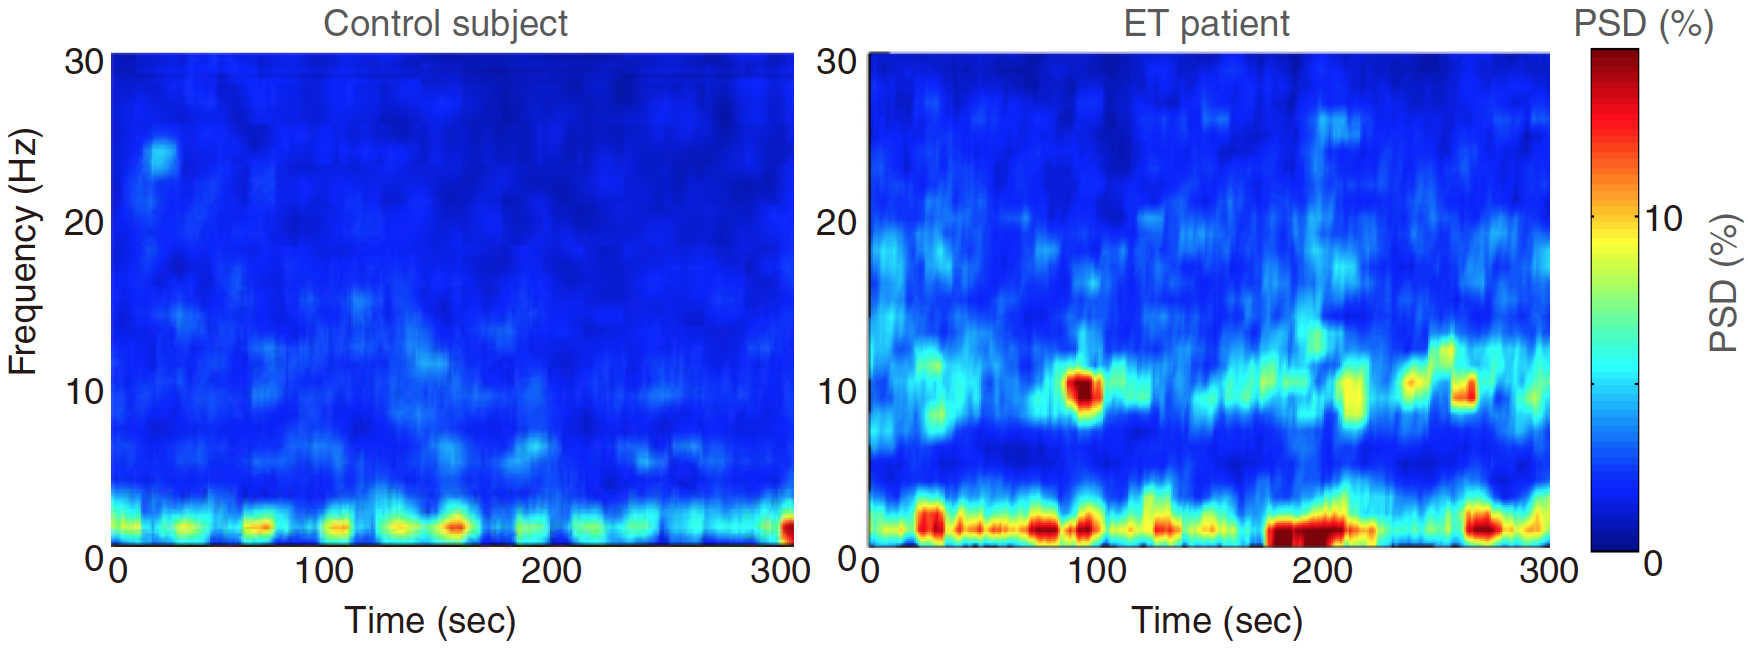
\includegraphics[width=0.9\textwidth]{et}
     \caption{مقایسه تحلیل فرکانسی نوسانات مغزی بیمار مبتلا به لرزش اساسی و نمونه کنترل }
     \label{fig:et-time-freq-analysis}
\end{figure}

اتفاق تقریبا مشابهی برای بیماری های دیگر نظیر پارکینسون، صرع و موارد دیگر نیز اتفاق می‌افتد. یکی از راه‌های درمانی برای مقابله با این شرایط استفاده از تحریک عمیق مغز می‌باشد. تحریک عمیق مغز به وسیله الکترودهایی که درون بافت مغز قرار می‌گیرند، اعمال می‌شود. همان‌طور که در شکل 
\ref{fig:dbs-xray}
پیداست، این الکترودها به کمک جراحی درون قسمت مشخصی از بافت مغز (منطقه هدف) کاشته می‌شوند. 

\begin{figure}
     \centering
     \begin{subfigure}[t]{0.3\textwidth}
         \centering
         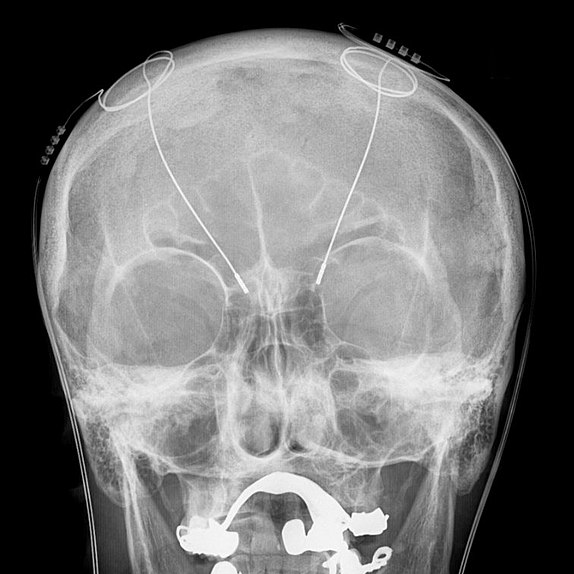
\includegraphics[width=\textwidth]{dbs-xray-1}
         \caption{الکترودهای تحریک عمیق مغز کاشته شده در سر }
%         \label{fig:tdcs}
     \end{subfigure}
     \
     %\hfill
     \begin{subfigure}[t]{0.3\textwidth}
         \centering
         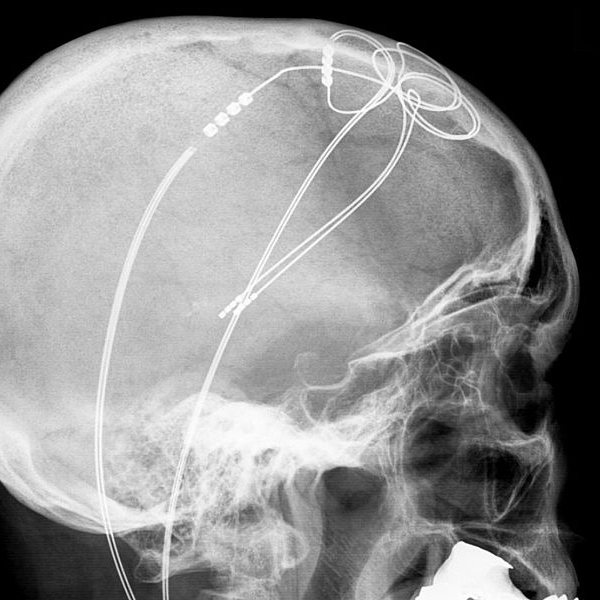
\includegraphics[width=\textwidth]{dbs-xray-2}
         \caption{الکترودهای تحریک عمیق مغز کاشته شده در سر }
%         \label{fig:tacs}
     \end{subfigure}
     \
  %   \hfill
     \begin{subfigure}[t]{0.3\textwidth}
         \centering
         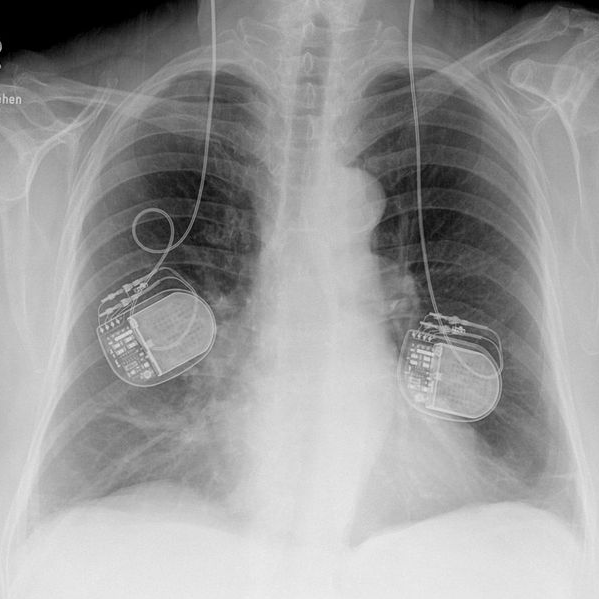
\includegraphics[width=\textwidth]{dbs-xray-3}
         \caption{    نوسان‌سازهای کار گذاشته شده درون قفسه سینه}
%         \label{fig:trns}
     \end{subfigure}
        \caption{
تصویر رادیولوژی سر و قفسه سینه فردی بعد از کاشت الکترودهای تحریک عمیق مغز.
         }
        \label{fig:dbs-xray}
\end{figure}

پس از کاشت الکترود، برای تضعیف نشانه‌های پاتولوژیک و ایجاد اثرات جانبی کمتر باید تعدادی پارامتر تحریک تنظیم شوند. مدل‌های محاسباتی برای تخمین پارامترهای بهینه تحریک عمیق مغز یاری دهنده هستند. در طول سال‌های گذشته پروتکل‌های مختلفی برای نحوه اعمال تحریک‌ها ارایه شده است که برخی از آن‌ها در شکل
\ref{fig:dbs-protocols}
نمایش داده شده‌اند.

\begin{figure}
	\centering
	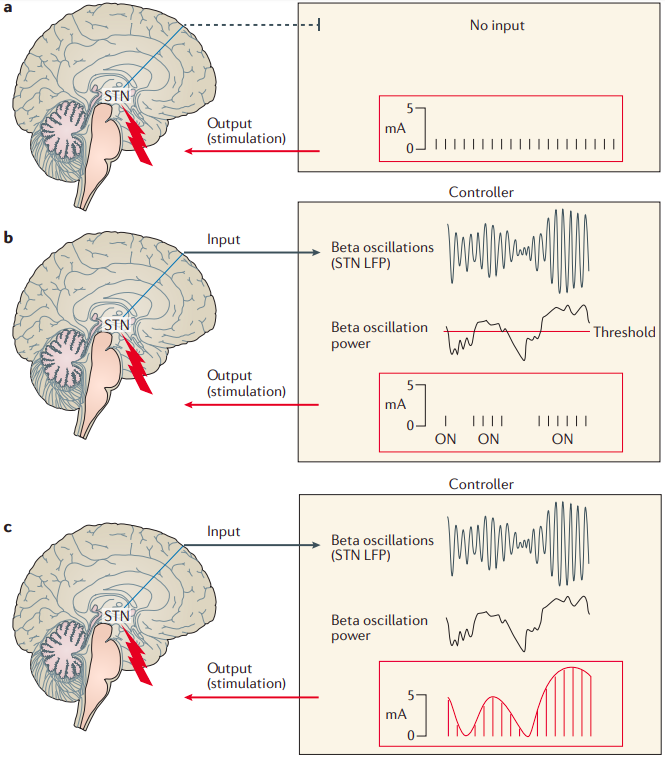
\includegraphics[width=0.9\textwidth]{dbs-protocols}
    \caption{
    پروتکل‌های مختلف در اعمال تحریک عمیق مغز.
در شکل بالایی تحریک عمیق مغز حلقه-باز را می‌بینیم؛ در این پروتکل پارامترهای تحریک ثابت هستند. از منظر فرکانس، تحریک عمیق مغز حلقه-باز دو دسته دارد. اگر فرکانس اعمال تحریک از ۱۰۰ هرتز کمتر باشد، فرایند تحریک در دسته تحریک عمیق مغز فرکانس پایین جای می‌گیرد و اگر فرکانس تحریک بیشتر از ۱۰۰ هرتز باشد فرآیند تحریک در دسته تحریک عمیق مغز با فرکانس بالا قرار می‌گیرد. اگر تحریک عمیق مغز با پارامتر‌های غیر ثابت، واکنشی و بر اساس تقاضا اعمال شود، تحریک عمیق مغز حلقه-بسته نامیده می‌شود. تحریک حلقه-بسته را می‌توان بر اساس نشانگرهای مختلفی اعمال کرد. برای مثال در شکل میانی، بر اساس پایش و نظارت یک پارامتر از سیگنال ورودی (در اینجا توان سیگنال ورودی)، خروجی دستگاه کنترل‌کننده را تعیین می‌کند. در پروتکل نشان داده شده در شکل میانی، تحریک هایی با دامنه ثابت، بر اساس اینکه آیا توان امواج بتا از آستانه مشخصی عبور کرده است یا خیر، به مغز اعمال می‌شود.
در پروتکل‌های مختلف ممکن است از بیش از یک مشخصه از سیگنال ورودی روی تعیین نحوه و مشخصات اعمال تحریک اثر بگذارد. مثلا در شکل پایین، قدرت تحریک نیز بر اساس قدرت سیگنال ورودی تنظیم می‌شود.
    }
    \label{fig:dbs-protocols}
\end{figure}

پارامترهای شکل موج از پارامترهای مهم در تحریک عمیق مغز می‌باشد. گروه‌های زیادی به بررسی نحوه اثر و پیدا کردن پارامترهای بهینه شکل موج می‌پردازند. در شکل 
\ref{fig:dbs-pulse-shape}
می‌توانید نمونه‌هایی از شکل موج‌های مختلف را مشاهده کنید. شکل موج بهینه می‌تواند اثرات جانبی را کاهش داده، احتمال آسیب دیدن بافت و الکترود را کم کند و همچنین طول عمر باتری را افزایش دهد. 


\begin{figure}
     \centering
     \begin{subfigure}[t]{0.3\textwidth}
         \centering
         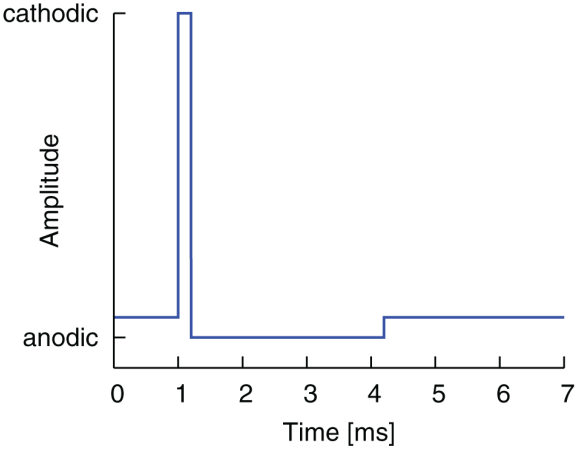
\includegraphics[width=\textwidth]{pulse-shape1}
%         \caption{الکترودهای تحریک عمیق مغز کاشته شده در سر }
%         \label{fig:tdcs}
     \end{subfigure}
     \
     %\hfill
     \begin{subfigure}[t]{0.3\textwidth}
         \centering
         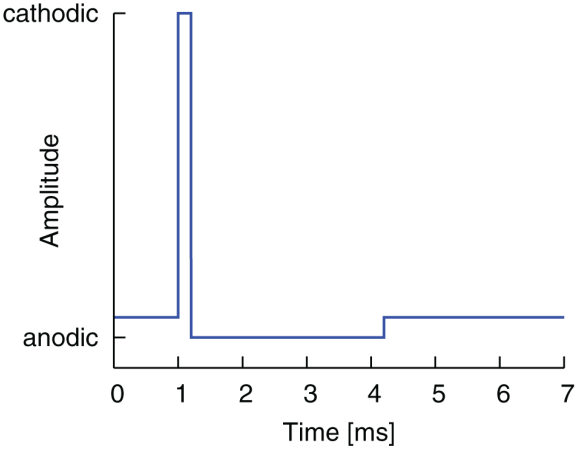
\includegraphics[width=\textwidth]{pulse-shape1}
%         \caption{الکترودهای تحریک عمیق مغز کاشته شده در سر }
%         \label{fig:tacs}
     \end{subfigure}
     \
  %   \hfill
     \begin{subfigure}[t]{0.3\textwidth}
         \centering
         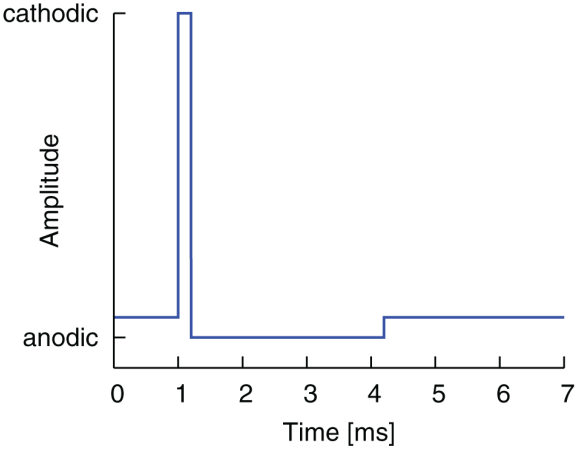
\includegraphics[width=\textwidth]{pulse-shape1}
%         \caption{    نوسان‌سازهای کار گذاشته شده درون قفسه سینه}
%         \label{fig:trns}
     \end{subfigure}
        \caption{
شکل موج‌های مختلف در تحریک عمیق مغز که بین قسمت‌های آنُدیک و کاتُدیک تاخیر متفاوتی دارند.
         }
        \label{fig:dbs-pulse-shape}
\end{figure}


رهیافت حلقه-بسته به اعمال تحریک براساس فعالیت در حال انجام مغز است. این رهیافت می‌تواند اثرات جانبی را کاهش داده و اثربخشی درمان را افزایش می‌دهد.


\begin{figure}
     \centering
     \begin{subfigure}[t]{0.45\textwidth}
         \centering
         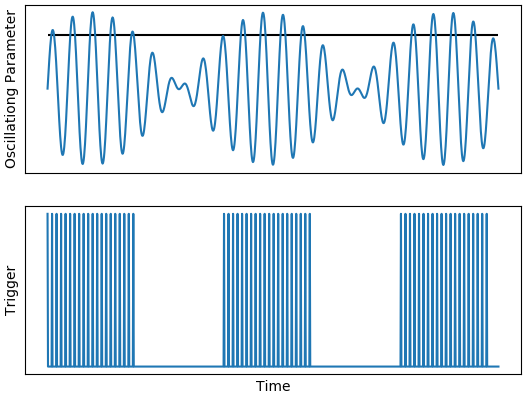
\includegraphics[width=\textwidth]{dbs-closedloop1}
         \caption{
         رهیافت حلقه-بسته، اعمال تحریک بر اساس دامنه فعالیت نوسانی در حال انجام در مغز.
         }
%         \label{fig:tdcs}
     \end{subfigure}
     \
     %\hfill
     \begin{subfigure}[t]{0.45\textwidth}
         \centering
         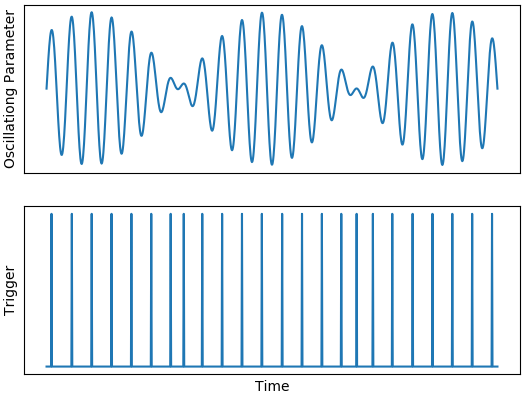
\includegraphics[width=\textwidth]{dbs-closedloop2}
         \caption{
         رهیافت حلقه-بسته، اعمال تحریک بر اساس فاز فعالیت نوسانی در حال انجام در مغز.
         }
%         \label{fig:tacs}
     \end{subfigure}
        \caption{
رهیافت حلقه-بسته
         }
        \label{fig:dbs-closed-loop}
\end{figure}

موفقیت تحریک عمیق مغز حلقه-بسته به طراحی استراتژی تحریک بستگی دارد که بر اساس آن نوسانات عصبی تضعیف می‌شوند. یک گام مهم در این راستا، ساختن مدلی ریاضی است که بتواند پاسخ نوسانات عصبی به تحریک در حالت‌های مختلف مغز را توصیف کند.
ما در بررسی‌های اولیه جمعیت نورونی که نوسانات پاتولوژیک تولید می‌کند را با شبکه ای از نوسانگرهای جفت شده مدل‌سازی کردیم. معادله تحول این نوسانگرها بر اساس مدل کوراموتو نوشته شده است. همچنین تحریک‌ها در یک لحظه خاص وقتی که فاز سیستم مقدار مشخصی است به اندازه تابع پاسخ فاز هر نوسانگر به آن‌ها وارد می‌شود.

\begin{equation}
    \frac{d \theta_i}{dt} = \omega_i + \frac{k}{N} \sum_{j=1}^{N} \sin(\theta_j -\theta_i) + I \delta(t-t_{stim}) Z(\theta_i)
    \label{eq:kuramotoModelres}
\end{equation}

جمله اول، 
$\omega_i$
فرکانس طبیعی نوسانگر 
$i$ 
ام می باشد.
جمله دوم توصیف کننده برهمکنش بین نوسانگرهای مختلف است که 
$k$
ضریب جفت شدگی می‌باشد و قدرت جفت شدگی بین هر جفت نوسانگر و در نتیجه تمایل نوسانگرها برای همگامی را کنترل می کند. 
جمله سوم اثر تحریک را توصیف می کند؛ شدت تحریک توسط 
$I$
مشخص شده است و تابع 
$\delta(t-t_{stim})$
در همه زمان ها صفر است به جز در زمان هایی که تحریک اعمال می‌شود که برابر است با یک.
تابع پاسخ فاز یک نوسانگر منفرد نیز
$Z(\theta_i)$
است.

\begin{figure}
	\centering
	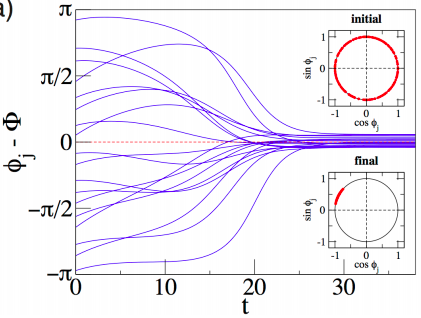
\includegraphics[width=0.45\textwidth]{kur100}
    \caption{
تحول زمانی فاز نوسانگرهای کوراموتو. در این شبیه‌سازی از ۱۰۰ نوسانگر استفاده شده است که فقط تحول زمانی فازهای ۱۸ عدد از نوسانگرها نمایش داده شده است. فرکانس ذاتی نوسانگرها به صورت تصادفی از توزیع نرمال (
$\mu=1.0$  و $\sigma=0.1$
) و فاز اولیه نوسانگرها نیز به صورت تصادفی از توزیع یکنواخت در بازه 
$[0,2\pi)$
انتخاب شده است. برای انتگرال‌گیری از روش اویلر با گام 
$dt\approx 0.01$
استفاده کرده‌ایم. واضح است که بعد از گذشت زمان همگامی نوسانگرها بیشتر شده است.
    }
%    \label{fig:dbs-protocols}
\end{figure}



\begin{figure}
	\centering
	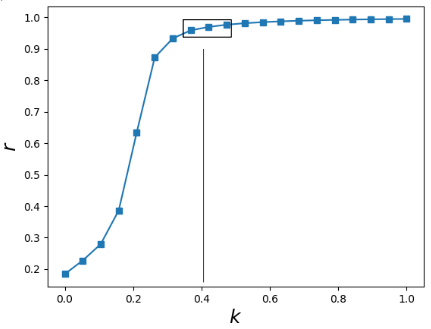
\includegraphics[width=0.45\textwidth]{kur1000orderParam}
    \caption{
نمودار اندازه پارامتر نظم بر حسب ضریب جفت شدگی. هر نقطه (برای هر مقدار ضریب جفت شدگی) از متوسط گیری پارامتر نظم ۴ سیستم با شرایط اولیه متفاوت تولید شده است. برای شبیه سازی هر سیستم از تعداد ۱۰۰۰ نوسانگر کوراموتو استفاده شده است. فرکانس ذاتی نوسانگرها به صورت تصادفی از توزیع نرمال (
$\mu=1.0$  و $\sigma=0.1$
) و فاز اولیه نوسانگرها نیز به صورت تصادفی از توزیع یکنواخت در بازه 
$[0,2\pi)$
انتخاب شده است. انتگرال‌گیری برای ۱۰۰۰ گام زمانی به طول
 $dt \approx 0.01$
 به روش اویلر انجام شده است که ۱۰ گام نهایی برای محاسبه پارامتر نظم آن سیستم میانگین گیری شده اند. محدوده مشخص شده در 
 $k \approx 0.4$
 محدوده مورد نطر ماست زیرا نوسانگرها به طور کامل همگام نمی‌شوند.
    }
    \label{fig:orderParam-k}
\end{figure}

اندازه پارامتر نظم معیاری از همگامی است؛ که مقادیر صفر و یک آن به ترتیب با حالت کاملا ناهمگام و حالت کاملا همگام متناظر هستند. وقتی تحریکی به سیستم وارد نشود، نوسانگرها تمایل به همگامی دارند. تمایل به همگامی توسط ضریب جفت شدگی کنترل می شود؛ به طوری که هرچه ضریب جفت شدگی بزرگ‌تر باشد همگامی سریع‌تر اتفاق میفتد. با توجه به اینکه ما در نظر داریم تحریک‌ را بر اساس فاز نوسانگرها اعمال کنیم، پس ضریب جفت شدگی را طوری انتخاب می‌کنیم که نوسانگرها کاملا همگام نشوند. بنابراین، با توجه به شکل 
\ref{fig:orderParam-k}
مقدار ضریب جفت‌شدگی 
$k \approx 0.4$
انتخاب می‌کنیم. در نهایت، بر اساس معادله تحول 
\ref{eq:kuramotoModelres}
در زمان‌های مختلف سیستم را تحریک می‌کنیم.

\begin{figure}
	\centering
	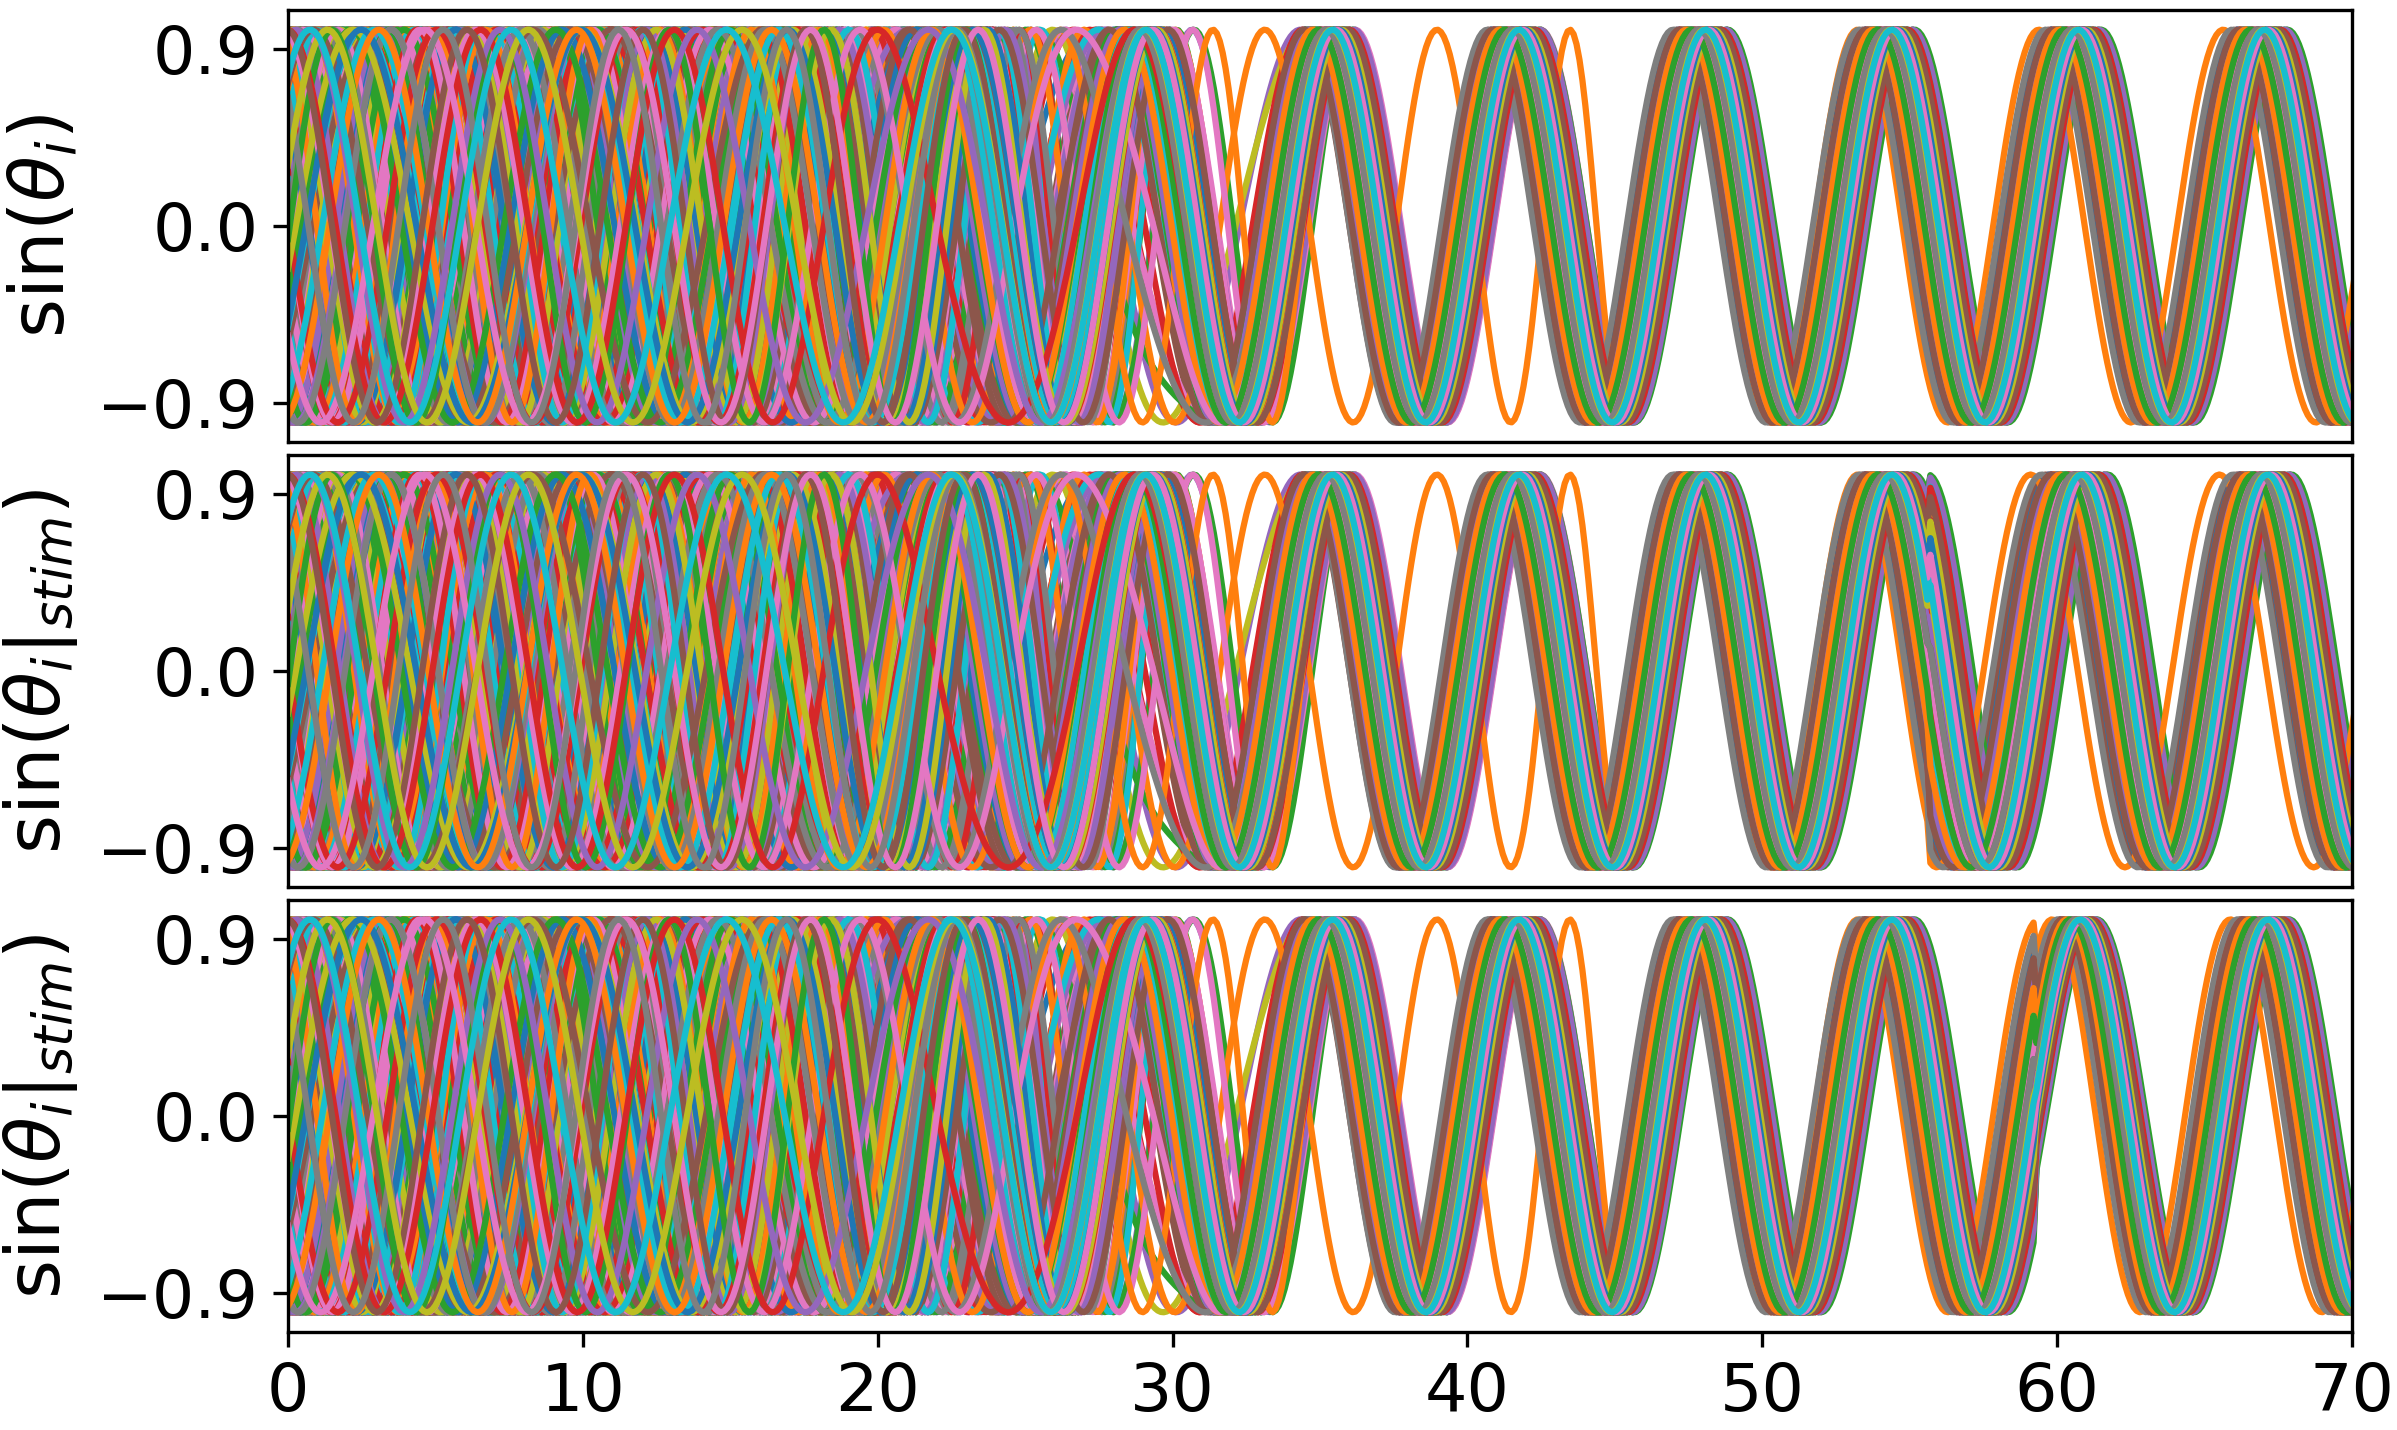
\includegraphics[width=0.9\textwidth]{kur1000-compare-thetas}
    \caption{
نمودار تحول فاز نوسانگرها در سه حالت مختلف. نمودار بالایی بدون اعمال تحریک. در نمودار میانی تحریک در لحظه 
$t=55.7$
و در نمودار پایینی در لحظه 
$t=59.3$
اعمال شده است.
    }
    \label{fig:kur-compare-thetas}
\end{figure}

در مورد شکل ها صحبت کن و دلتا ار رو معرفی کن.!!!!!!!!!!!!!!!!!!!!!!!!!!!!!!!!!!

\begin{figure}
     \centering
     \begin{subfigure}[t]{0.3\textwidth}
         \centering
         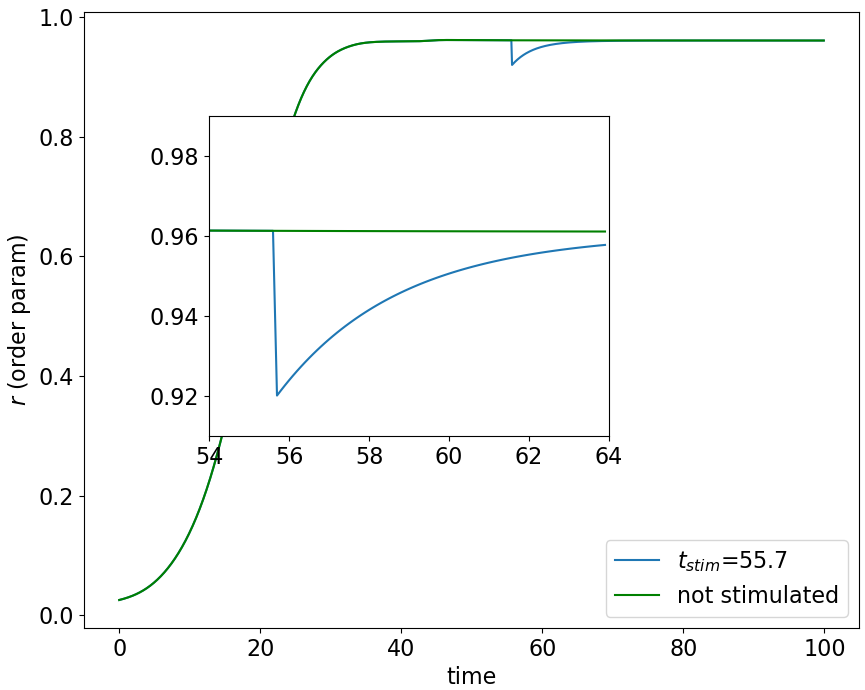
\includegraphics[width=\textwidth]{k1000stim-orderParam1}
%         \caption{الکترودهای تحریک عمیق مغز کاشته شده در سر }
%         \label{fig:tdcs}
     \end{subfigure}
     \
     %\hfill
     \begin{subfigure}[t]{0.2\textwidth}
         \centering
         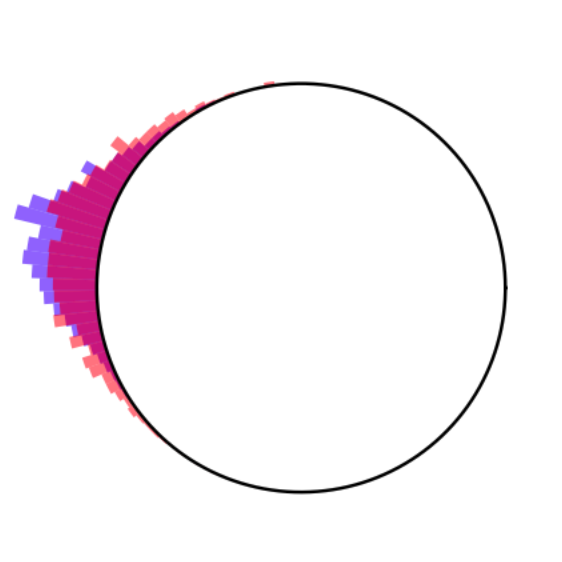
\includegraphics[width=\textwidth]{distro1}
%         \caption{الکترودهای تحریک عمیق مغز کاشته شده در سر }
%         \label{fig:tacs}
     \end{subfigure}
     \
  %   \hfill
     \begin{subfigure}[t]{0.4\textwidth}
         \centering
         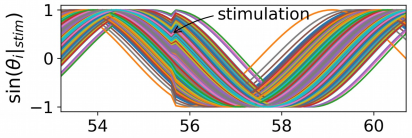
\includegraphics[width=\textwidth]{k1000theta-stim1}
%         \caption{    نوسان‌سازهای کار گذاشته شده درون قفسه سینه}
%         \label{fig:trns}
     \end{subfigure}
        \caption{
اعمال تحریک در لحظه 
$t=55.7$.
در شکل سمت چپ نمودار تحول زمانی فاز نوسانگرها را مشاهده می‌کنیم. در شکی میانی توزیع فاز در لحظه های قبل (آبی) و بعد (قرمز) از اعمال تحریک را می‌بینیم و در شکل سمت راست تحول زمانی پارامتر نظم برای سیستم تحریک شده (آبی) و سیستم تحریک نشده  (سبز).
         }
%        \label{fig:dbs-xray}
\end{figure}

\begin{figure}
     \centering
     \begin{subfigure}[t]{0.3\textwidth}
         \centering
         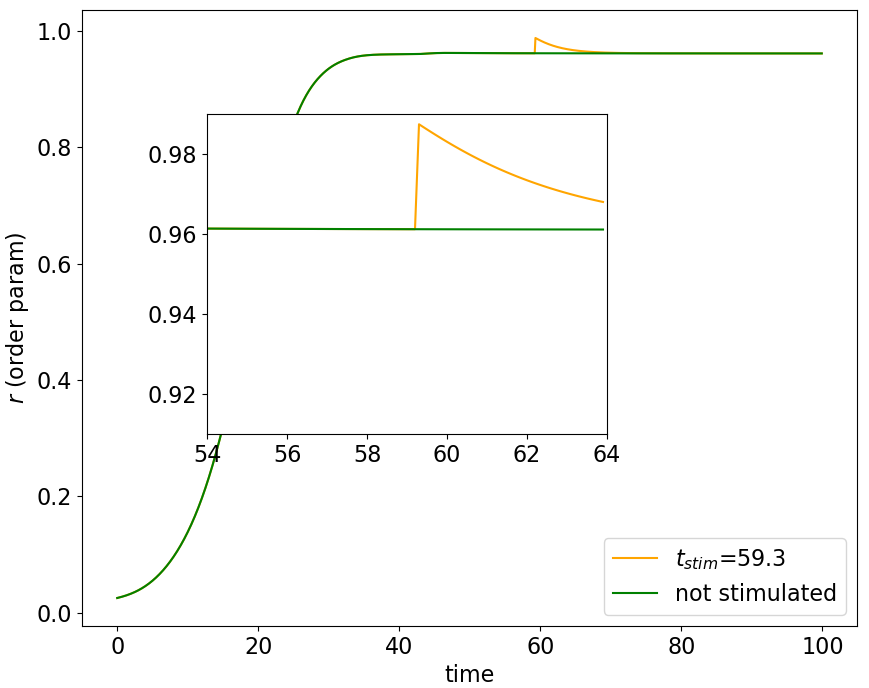
\includegraphics[width=\textwidth]{k1000stim-orderParam2}
%         \caption{ تحول زمانی پارامتر نظم }
%         \label{fig:tdcs}
     \end{subfigure}
     \
     %\hfill
     \begin{subfigure}[t]{0.2\textwidth}
         \centering
         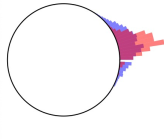
\includegraphics[width=\textwidth]{distro2}
%         \caption{فراوانی فاز نوسانگرها قبل و بعد از تحریک }
%         \label{fig:tacs}
     \end{subfigure}
     \
  %   \hfill
     \begin{subfigure}[t]{0.4\textwidth}
         \centering
         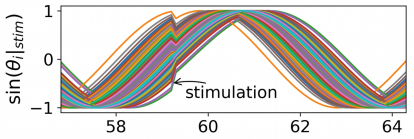
\includegraphics[width=\textwidth]{k1000theta-stim2}
%         \caption{تحول زمانی فاز نوسانگرها }
%         \label{fig:trns}
     \end{subfigure}
        \caption{
اعمال تحریک در لحظه 
$t=59.3$.
در شکل سمت چپ نمودار تحول زمانی فاز نوسانگرها را مشاهده می‌کنیم. در شکی میانی توزیع فاز در لحظه های قبل (آبی) و بعد (قرمز) از اعمال تحریک را می‌بینیم و در شکل سمت راست تحول زمانی پارامتر نظم برای سیستم تحریک شده (نارنجی) و سیستم تحریک نشده  (سبز).
         }
%        \label{fig:dbs-xray}
\end{figure}



\begin{figure}
	\centering
	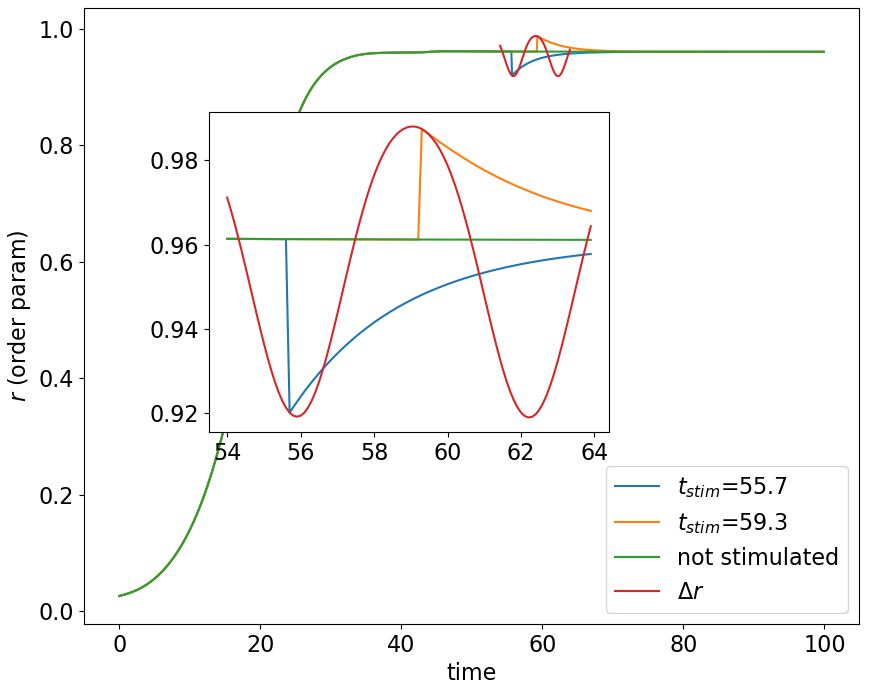
\includegraphics[width=0.5\textwidth]{k1000stim-orderParam}
    \caption{
بیشینه تغییرات پارامتر نظم سیستم تحریک شده و سیستم تحریک نشده بر حسب زمان اعمال تحریک.
    }
%    \label{fig:kur-compare-thetas}
\end{figure}




\begin{figure}
	\centering
	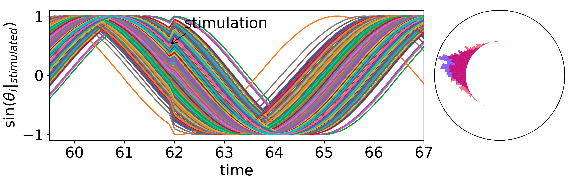
\includegraphics[width=0.7\textwidth]{theta-dist}
    \caption{
اعمال تحریک در لحظه 
$t=61.9$.
    }
%    \label{fig:kur-compare-thetas}
\end{figure}



\begin{figure}
	\centering
	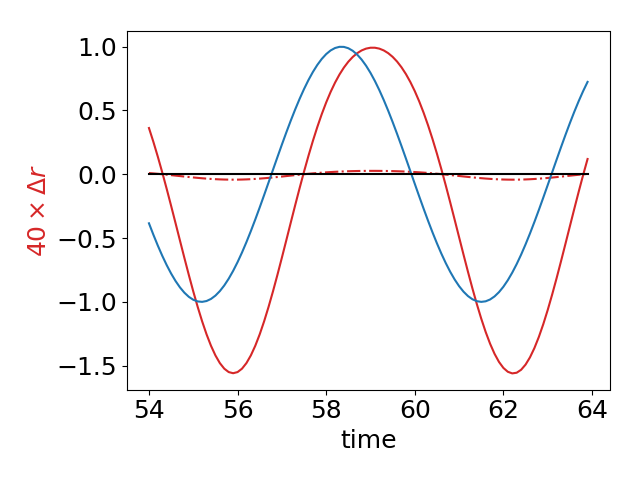
\includegraphics[width=0.6\textwidth]{orderParam-prc}
    \caption{
نمودار بیشینه تغییرات پارامتر نظم بین سیستم تحریک شده و تحریک نشده (خط نقطه قرمز) و تابع پاسخ فاز جمعیت (آبی).
    }
%    \label{fig:kur-compare-thetas}
\end{figure}

\begin{figure}
	\centering
	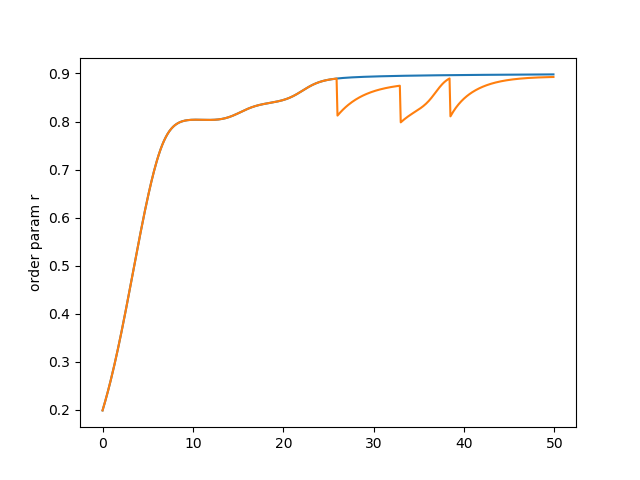
\includegraphics[width=0.6\textwidth]{multiple-stim}
    \caption{
با اعمال تحریک‌های پیاپی بر اساس فاز سیستم در دوره‌های مختلف می‌توان پارامتر نظم را کاهش داد و همچنین حالت دینامیکی سیستم را نیز تغییر داد.
    }
%    \label{fig:kur-compare-thetas}
\end{figure}

نوسانات همگام درون و بین نواحی مغز به پردازش عادی اطلاعات در مغز کمک می‌کنند؛ اما در برخی از بیماری‌های سیستم عصبی، این نوسانات در مقایسه با مغز سالم تقویت می‌شوند. به عنوان مثال می‌توان به نوسانات تقویت شده بتا (با فرکانس تقریبی ۲۰ هرتز) که بین قشر و هسته زیرتالاموسی در بیماران پارکینسونی ثبت شده است، اشاره کرد. تحریکِ عمیقِ مغز، درمانی مؤثر برای اختلالات عصبی متنوعی از جمله پارکینسون و لرزش اساسی است. در حال حاضر در روش تحریک عمیق مغز، قطاری از پالس‌های الکتریکی با بسامد ثابت توسط الکترود‌هایی که در مغز کاشته شده‌اند به محل‌های هدف در مغز اعمال می شوند.  تحریک عمیق مغز حلقه‌بسته یک رهیافت جدید و  امید‌بخش است که تحریک بر اساس وضعیت بیمار اعمال می‌شود. در این رهیافت جدید به جای آنکه از قطاری از پالس‌های با بسامد ثابت استفاده کنند، تحریک بر اساس فعالیت مغزی بیمار اعمال می‌شود.  این روش توانایی زیادی برای پیشرفت در بهره‌وری، ثمربخشی و کاهش اثرات جانبی دارد. بهبود این روش وابسته به ابداع کردن یک راهبرد تحریک است که نوسانات فعالیت‌های عصبی که نشانه بیماری هستند را کاهش دهد. یکی از راه‌های رسیدن به این هدف مدل سازی‌های نظری و محاسباتی است. این مدل سازی‌ها توصیف خوبی از نحوه تغییر نوسانات مغزی بعد از اعمال تحریک ارایه می‌دهند. برای مثال، مدل سازی های محاسباتی پیشنهاد می کنند که دامنه نوساناتی که نشانه بیماری هستند را می توان با اعمال تحریک در فازهای مشخصی از نوسانات، اصلاح کرد. در این مطالعه، در نواحی‌ای که نوسانات نشانه بیماری را تولید می‌کنند به جای نورون‌ها از نوسانگر های جفت شده استفاده می‌کنیم و نشان می دهیم که اگر در فاز و دامنه مشخصی تحریک را اعمال کنیم، سیستم عصبی چطور به آن تحریک پاسخ خواهد داد. همچنین نشان می‌دهیم که با توجه به منحنی پاسخ فاز نوسانگرها می‌توان بهترین زمان اعمال پالس را برای بیشترین کاهش در دامنه نوسان پیش‌بینی کرد.